\documentclass{article}
\usepackage{amsmath, amssymb, amsthm, graphicx}
\usepackage[export]{adjustbox}

\title{Chapter 2 Section 2}
\author{Andrew Taylor}
\date{April 6 2022}
\newtheorem{theorem}{Theorem}
\newtheorem{problem}{Problem}
\newtheorem*{solution}{Solution}

\begin{document}
\maketitle

The letter L can be represented by the vectors $(0, 2)$ and $(1, 0)$. 

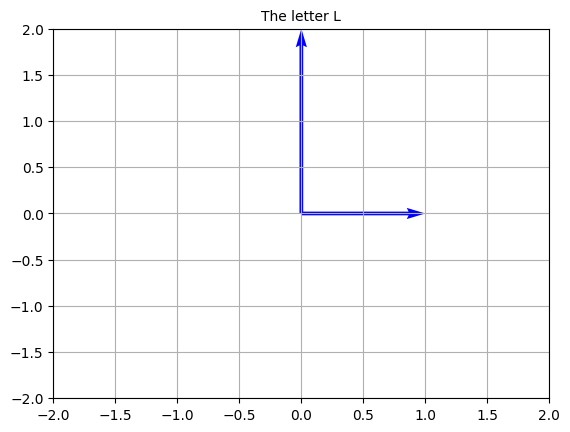
\includegraphics[scale=0.5, center]{L} 

The following problems ask for a linear transformation of the letter L. In the following problems, give the matrix of the transformation and plot the result.

\begin{problem}
Scale L by a factor of $\displaystyle \frac{1}{2}$
\end{problem}

\begin{solution}
The matrix of the transformation is 

\begin{align*}
\begin{bmatrix}
0.5 & 0.0 \\ 
0.0 & 0.5
\end{bmatrix}
\end{align*}

After the scaling, the L looks like this

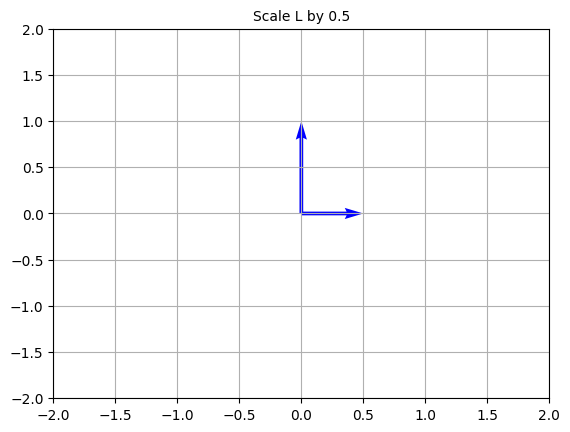
\includegraphics[scale=0.5, center]{Lscalebyhalf} 

Note that in creating this shape, we scaled both vectors that make up the L.

\end{solution}

\begin{problem}
Rotate L ninety degrees counterclockwise
\end{problem}

\begin{solution}
The matrix of the transformation is 

\begin{align*}
\begin{bmatrix}
0 & -1 \\ 
1 & 0
\end{bmatrix}
\end{align*}

After the rotation, the L looks like this

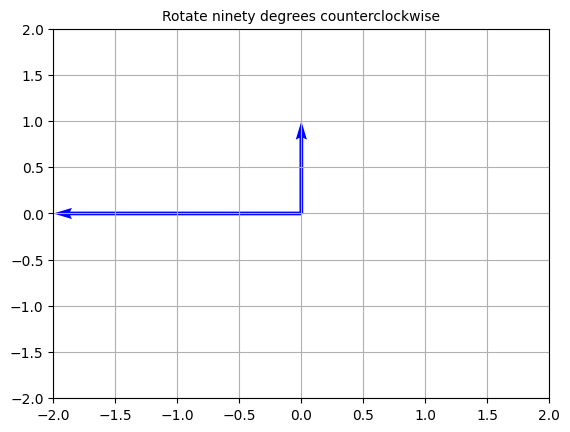
\includegraphics[scale=0.5, center]{Lrot90} 

\end{solution}

\begin{problem}
Reflect L about the Y axis
\end{problem}

\begin{solution}
The matrix of the transformation is

\begin{align*}
\begin{bmatrix}
-1 & 0 \\ 
0 & 1
\end{bmatrix}
\end{align*}

The plot looks like this

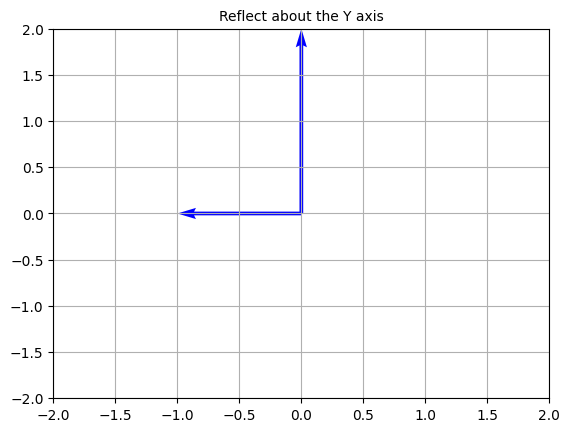
\includegraphics[scale=0.5, center]{Lreflecty} 

\end{solution}

\begin{problem}
Reflect L about the X axis
\end{problem}

\begin{solution}
The matrix of the transformation is 

\begin{align*}
\begin{bmatrix}
0 & 1 \\ 
-1 & 0
\end{bmatrix}
\end{align*}

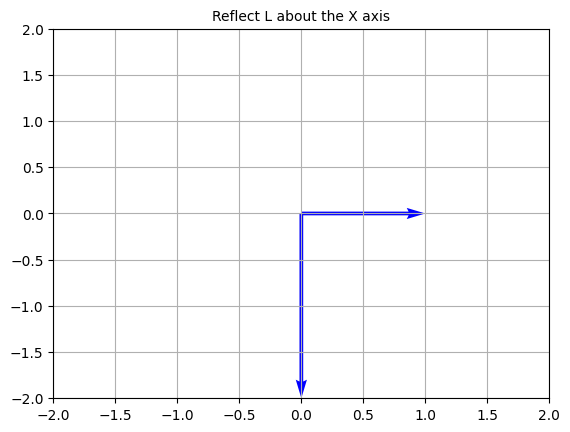
\includegraphics[scale=0.5, center]{Lreflectx} 

\end{solution}

\begin{problem}
Rotate L forty five degrees counterclockwise
\end{problem}

\begin{solution}
The matrix of the transformation is 

\begin{align*}
\begin{bmatrix}
\cos(\frac{\pi}{4}) & -1 * \sin(\frac{\pi}{4}) \\ 
\sin(\frac{\pi}{4}) & \cos(\frac{\pi}{4})
\end{bmatrix}
\end{align*}

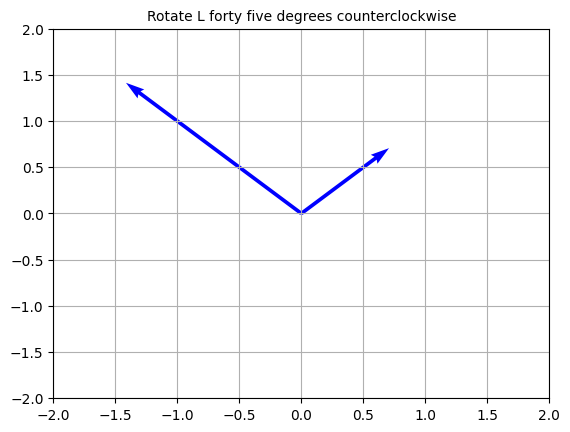
\includegraphics[scale=0.5, center]{Lrot45} 
\end{solution}

\begin{problem}
Find the orthogonal projection of L onto the x-axis
\end{problem}

\begin{solution}
The matrix of the transformation is 

\begin{align*}
\begin{bmatrix}
1 & 0 \\ 
0 & 0
\end{bmatrix}
\end{align*}

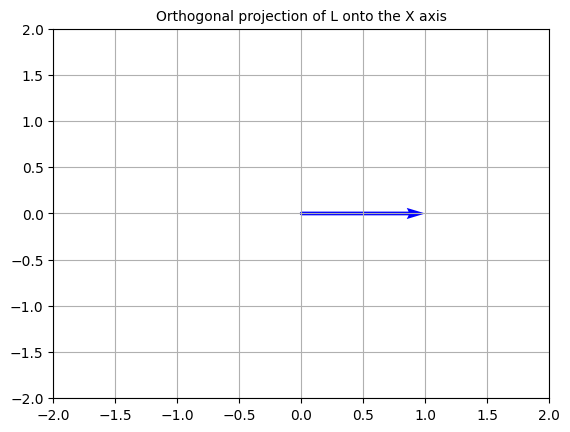
\includegraphics[scale=0.5, center]{Lorthogonalprojx} 

\end{solution}

\begin{problem}
Find the orthogonal projection of L onto the y-axis
\end{problem}

\begin{solution}
The matrix of the transformation is 

\begin{align*}
\begin{bmatrix}
0 & 0 \\ 
0 & 1
\end{bmatrix}
\end{align*}

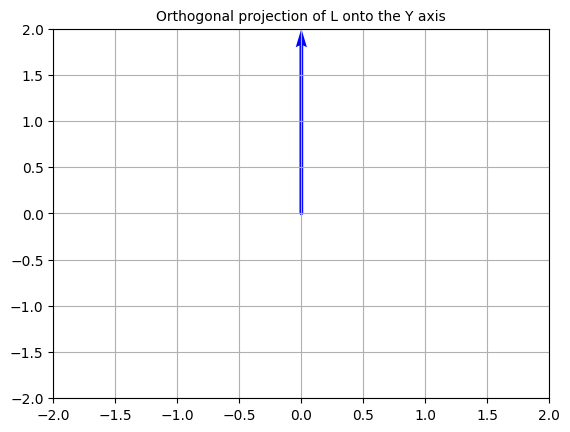
\includegraphics[scale=0.5, center]{Lorthogonalprojy} 

\end{solution}

\begin{problem}
Find the matrix P of the orthogonal projection onto the line L spanned by $\vec{w} = \begin{pmatrix} 3 \\ 4 \end{pmatrix}$
\end{problem}

\begin{solution}
\begin{align*}
P &= 
\displaystyle \frac{1}{w_{1}^2 + w_{2}^2} 
\begin{bmatrix}
w_{1}^2 & w_{1}w_{2} \\
w_{1}w_{2} & w_{2}^2
\end{bmatrix} \\
&=
\displaystyle \frac{1}{25} 
\begin{bmatrix}
9 & 12 \\
12 & 16
\end{bmatrix} \\
&= 
\begin{bmatrix}
0.36 & 0.48 \\
0.48 & 0.64
\end{bmatrix}
\end{align*}
\end{solution}

\end{document}